%! Author = sriadityavedantam
%! Date = 4/7/26

\section{Rational Maps}

Let $X,Y$ be irreducible plane curves.
Recall that if $u = \frac{p}{q}\in\c(X)$, then $u$ is defined at all but finitely many points of $X$.
Thus we may view
\[
    u : X \dashrightarrow \aa^1.
\]

Given $u,v\in\c(X)$, we get a rational map
\[
    (u,v) : X \dashrightarrow \aa^2.
\]

\begin{definition}[Rational Map]
    A map $\varphi : X \dashrightarrow Y$ is rational if and only if there exist rational functions $u,v\in\c(X)$ such that $(u,v): X \dashrightarrow \aa^2$ factors through $Y$.
    \begin{figure}[H]
        \centering
        \tikzset{every picture/.style={line width=0.75pt}}
        \colorbox{white}{%
            \color{black}
            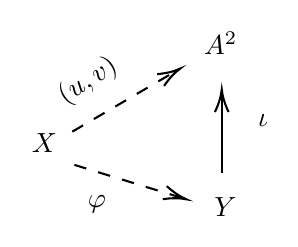
\begin{tikzpicture}[
                x=0.75pt,
                y=0.75pt,
                yscale=-1,
                xscale=1,
                every node/.style={text=black},
                every path/.style={draw=black},
                line width=0.75pt
            ]
                \draw  [dash pattern={on 4.5pt off 4.5pt}]  (266,115) -- (316.27,85.61) ;
                \draw [shift={(318,84.6)}, rotate = 149.69] [color={rgb, 255:red, 0; green, 0; blue, 0 }][line width=0.75] (10.93,-3.29) .. controls (6.95,-1.4) and (3.31,-0.3) .. (0,0) .. controls (3.31,0.3) and (6.95,1.4) .. (10.93,3.29) ;
                \draw  [dash pattern={on 4.5pt off 4.5pt}]  (267,131) -- (319.09,147.01) ;
                \draw [shift={(321,147.6)}, rotate = 197.09] [color={rgb, 255:red, 0; green, 0; blue, 0 }][line width=0.75] (10.93,-3.29) .. controls (6.95,-1.4) and (3.31,-0.3) .. (0,0) .. controls (3.31,0.3) and (6.95,1.4) .. (10.93,3.29) ;
                \draw    (338,135) -- (338,96.6) ;
                \draw [shift={(338,94.6)}, rotate = 90] [color={rgb, 255:red, 0; green, 0; blue, 0 }][line width=0.75] (10.93,-3.29) .. controls (6.95,-1.4) and (3.31,-0.3) .. (0,0) .. controls (3.31,0.3) and (6.95,1.4) .. (10.93,3.29) ;

                \draw (245,114.4) node [anchor=north west][inner sep=0.75pt] {$X$};
                \draw (254.92,92.94) node [anchor=north west][inner sep=0.75pt] [rotate=-327.11] {$(u,v)$};
                \draw (328,65.4) node [anchor=north west][inner sep=0.75pt] {$\mathbb{A}^{2}$};
                \draw (272,144.4) node [anchor=north west][inner sep=0.75pt] {$\varphi$};
                \draw (333,145.4) node [anchor=north west][inner sep=0.75pt] {$Y$};
                \draw (354,105.4) node [anchor=north west][inner sep=0.75pt] {$\iota$};
            \end{tikzpicture}
        }
    \end{figure}
    Thus
    \[
        (u,v) = \iota\circ\varphi,
    \]
    that is,
    \[
        \ima(u,v)\subseteq Y.
    \]
\end{definition}

\begin{remark}
    If $C$ is a rational curve, then there is a rational map
    \[
        \aa^1 \dashrightarrow C.
    \]
    That is, if $C : \{f(x,y)=0\}\subseteq \aa^2$, then a rational parametrization has the form
    \[
        x = u(t), \qquad y = v(t)
    \]
    for some rational functions $u(t),v(t)\in\c(t)$.
\end{remark}

Let the line $\ell\subseteq \aa^2$.
Let $P\in \aa^2$ be a point with $P\notin \ell$.

\begin{figure}[H]
    \centering
    \tikzset{every picture/.style={line width=0.75pt}}
    \colorbox{white}{%
        \color{black}
        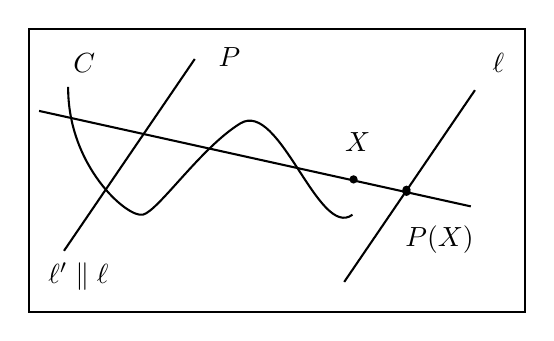
\begin{tikzpicture}[
            x=0.75pt,
            y=0.75pt,
            yscale=-1,
            xscale=1,
            every node/.style={text=black},
            every path/.style={draw=black},
            line width=0.75pt
        ]
            \draw   (201,46) -- (440.05,46) -- (440.05,182.6) -- (201,182.6) -- cycle ;
            \draw    (220,74) .. controls (219.75,112.18) and (248.6,137.32) .. (256,135.6) .. controls (263.4,133.88) and (284.12,103.1) .. (303,91.6) .. controls (321.88,80.1) and (340.64,147.87) .. (357,135.6) ;
            \draw    (353,168) -- (416,75.6) ;
            \draw    (206,85.6) -- (414,131.6) ;
            \draw    (218,153) -- (281,60.6) ;
            \draw  [line width=3] [line join = round][line cap = round] (357.5,118.6) .. controls (357.5,118.6) and (357.5,118.6) .. (357.5,118.6) ;
            \draw  [line width=3] [line join = round][line cap = round] (383,124.6) .. controls (383,124.6) and (383,124.6) .. (383,124.6) ;
            \draw  [line width=3] [line join = round][line cap = round] (383,123.6) .. controls (383,123.6) and (383,123.6) .. (383,123.6) ;

            \draw (209,157.4) node [anchor=north west][inner sep=0.75pt] {$\ell' \parallel \ell$};
            \draw (291,53.4) node [anchor=north west][inner sep=0.75pt] {$P$};
            \draw (221,56.4) node [anchor=north west][inner sep=0.75pt] {$C$};
            \draw (352,94.4) node [anchor=north west][inner sep=0.75pt] {$X$};
            \draw (381,139.4) node [anchor=north west][inner sep=0.75pt] {$P(X)$};
            \draw (423,56.4) node [anchor=north west][inner sep=0.75pt] {$\ell$};
        \end{tikzpicture}
    }
\end{figure}

Consider the projection map
\begin{gather*}
    P : \aa^2\setminus \ell' \to \ell,\\
    x \mapsto P(x).\\
\end{gather*}

Then we may consider the restriction
\[
    P|_C : C \dashrightarrow \ell,
\]
where $C$ is any irreducible curve.

\begin{definition}[Birational]
    A rational map $\varphi : X \dashrightarrow Y$ is birational if and only if there exists a rational map $\psi : Y \dashrightarrow X$ satisfying
    \begin{enumerate}[label={(\arabic*)}]
    \item $\varphi\circ\psi = \Id_Y$,
    \item $\psi\circ\varphi = \Id_X$,
    \end{enumerate}
    whenever defined.
\end{definition}

We call two curves birational if and only if there exists a birational map between them.

\begin{theorem}{
    $X$ is rational if and only if $\c(X)\cong \c(t)$.
}
If $X$ is rational, then $X$ is birational to $\aa^1$.
A birational map induces an isomorphism of function fields, so
\[
    \c(X)\cong \c(\aa^1)=\c(t).
\]

Conversely, suppose $\c(X)\cong \c(t)$.
Then $\c(X)$ is isomorphic to a purely transcendental extension of degree $1$.
By Lüroth's Theorem, the intermediate field comes from a single rational parameter.
Hence $X$ is birational to $\aa^1$, so $X$ is rational.
\end{theorem}

\begin{theorem*}[Lüroth's Theorem]{
    Let $K\subseteq \c(t)$ be a subfield with $\c\subseteq K$.
    Then there exists $r(t)\in\c(t)$ such that
    \[
        K = \c(r(t)).
    \]
}
\end{theorem*}